\documentclass[../portafolio.tex]{subfiles}

\begin{document}

\chapter{introduccion a Python}
\label{ch:ejercicios-python}

\chapterauthor{Bruno Bustos, Camilo Jordan}

\hfill \textbf{Fecha de la actividad:} 8 de septiembre de 2025

\medskip

%aqui una introdiuccion al capitulo

En este capitulo se resolveran los ejercicios proporcionados por el profesor, los
cuales abarcan conceptos basicos de python, demostraciones numericas y conceptuales.

\medskip

\section*{Conceptos basicos de python}



\section*{Funciones de Numpy}



\section*{Numeros de Catalan}

Los numeros de Catalan son una secuencia de numeros naturales que tienen muchas aplicaciones en combinatoria
y teoria de grafos. Se definen mediante la siguiente manera:

\begin{equation}
    C_n = \frac{(2n)!}{(n+1)!n!}
\end{equation}

Ahora, mediante el uso de esa formula podremos calcular los primeros 15 numeros de Catalan.
Utilizando funciones creadas mediante Python y Numpy, pero primero debemos definir el factorial de un numero.

\begin{lstlisting}
    def factorial(N):
        """Retorna una lista de factoriales desde 0! hasta N!. Por ejemplo:
            factorial(5) -> [1, 1, 2, 6, 24, 120]"""
        f = 1 #note el uso del operador walrus := a continuacion
        return [1 if n == 0 else (f := f * n) for n in range(N+1)]
\end{lstlisting}

Siendo este el codigo para calcular el factorial de un numero solo utilizando funciones de Python, Ahora con 
Numpy:

\begin{lstlisting}
    import numpy as np

    def factorial_numpy(N, dtype=np.int32):

    """Retorna un arreglo de numpy de factoriales desde 0! hasta N!.
        El argumento "dtype" controla la precisión. Ejemplos:
        factorial_numpy(5) -> array([1, 1, 2, 6, 24, 120], dtype=int32)
        factorial_numpy(5, dtype=np.int64) -> array([1, 1, 2, 6, 24, 120], dtype=int64)"""
    
    f = np.arange(N+1, dtype=dtype)
    f[0] = 1
    return f.cumprod(dtype=dtype)
\end{lstlisting}

Ahora, utilizando la funcion de factorial definida anteriormente definiremos otras funciones para calcular
otros factoriales necesarios para el calculo de los numeros de Catalan, como $(2n)!$ y $(n+1)!$.

\begin{lstlisting}
    # (2n)! factorial con python

def factorial_2n(N):
    f = 1
    return [1 if n==0 else (f:=f*(2*n-1)*(2*n)) for n in range(N+1)]

# (n+1)! factorial con python}

def factorial_n1(N):
    f = 1
    return [1 if n==0 else (f:=f*(n+1)) for n in range(N+1)]
\end{lstlisting}

Esto para la version con funciones de Python, y para la version con funciones de Numpy:

\begin{lstlisting}
    # (2n)! factorial con numpy

def factorial_2n_numpy(N, dtype=np.int32):
    f = np.arange(2*N+1, dtype=dtype)
    f[0] = 1
    return f.cumprod(dtype=dtype)[::2]

# (n+1)! factorial con numpy

def factorial_n1_numpy(N, dtype=np.int32):
    f = np.arange(N+2, dtype=dtype)
    f[0] = 1
    return f.cumprod(dtype=dtype)[1:]
\end{lstlisting}

Finalmente, con estas funciones ya definidas podemos calcular los numeros de Catalan con la formula dada \eqref{1}.
Con nuestro codigo final siendo el siguiente:

\begin{lstlisting}
    #Ahora calculamos y graficamos los numeros de catalan desde n=0 hasta n=15
    fac = factorial(N)        # lista de n!
    fac2n = factorial_2n(N)   # lista de (2n)!
    fac_n1 = factorial_n1(N)  # lista de (n+1)!

    #Usa la longitud de cualquiera de las listas, en este caso de n!
    L = len(fac)

    #Definimos la lista vacia para ir guardando los num de catalan
    cat=[]

    for i in range(L):
    cat.append(fac2n[i] // (fac[i] * fac_n1[i]))
print(cat)
\end{lstlisting}

Siendo este el codigo final para calcular los numeros de Catalan utilizando funciones de Python, y para la version
con Numpy:

\begin{lstlisting}
    #Ahora calculamos y graficamos los numeros de catalan desde n=0 hasta n=15
    fac = factorial_numpy(N, dtype=np.int32)        # lista de n!
    fac2n = factorial_2n_numpy(N, dtype=np.int32)   # lista
    fac_n1 = factorial_n1_numpy(N, dtype=np.int32)  # lista de (n+1)!

    #Usa la longitud de cualquiera de las listas, en este caso de n!
    L = len(fac)

    #Definimos la lista vacia para ir guardando los num de catalan
    cat=[]
    for i in range(L):
    cat.append(fac2n[i] // (fac[i] * fac_n1[i]))

    print(cat)  #podemos notar que por overflow nos da numeros negativos a partir de n=13
\end{lstlisting}

Mediante el uso de los codigos anteriores podemos obtener los primeros numeros de Catalan, pero notamos que 
en el codigo con Numpy a partir de $N=6$ los numeros comienzan a ser incorrectos, esto debido a que el tipo de dato
utilizado (int32) no es capaz de almacenar numeros tan grandes, por lo que debemos cambiar el tipo de dato a int64, 
para evitar este problema, y asi obtener los primeros 15 numeros de Catalan correctamente.
Pero en el codigo con funciones de Python no tenemos este problema, ya que Python maneja los enteros de manera
automatica, por lo que no tenemos que preocuparnos por el tipo de dato. Entonces, los primeros 15 numeros de Catalan 
son:

\begin{table}[ht]
\centering
\small 
\caption{Números de Catalán $C_n$ para $0\le n \le 15$}
\label{tab:catalan_0_15}
\begin{tabular}{@{}*{16}{c}@{}} 
$C_0$ & $C_1$ & $C_2$ & $C_3$ & $C_4$ & $C_5$ & $C_6$ & $C_7$
 & $C_8$ & $C_9$ & $C_{10}$ & $C_{11}$ & $C_{12}$ & $C_{13}$ & $C_{14}$ & $C_{15}$ \\[4pt]
1 & 1 & 2 & 5 & 14 & 42 & 132 & 429 & 1430 & 4862 & 16796 & 58786 & 208012 & 742900 & 2674440 & 9694845 \\
\end{tabular}
\end{table}

Ahora, graficando los numeros de Catalan obtenidos mediante los codigos anteriores tenemos que:

\begin{figure}[ht]
  \centering
  \begin{minipage}[b]{0.48\textwidth}
    \centering
    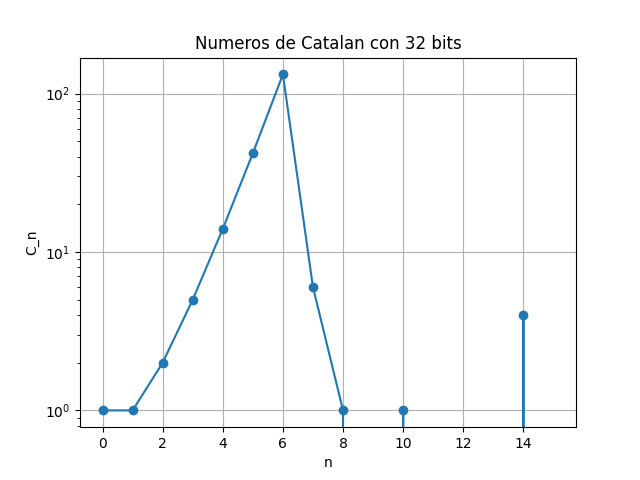
\includegraphics[width=\linewidth]{../img/Catalan_numpy32.png}
    \caption{Utilizando funciones de Numpy.}
    \label{fig:min1}
  \end{minipage}
  \hfill
  \begin{minipage}[b]{0.48\textwidth}
    \centering
    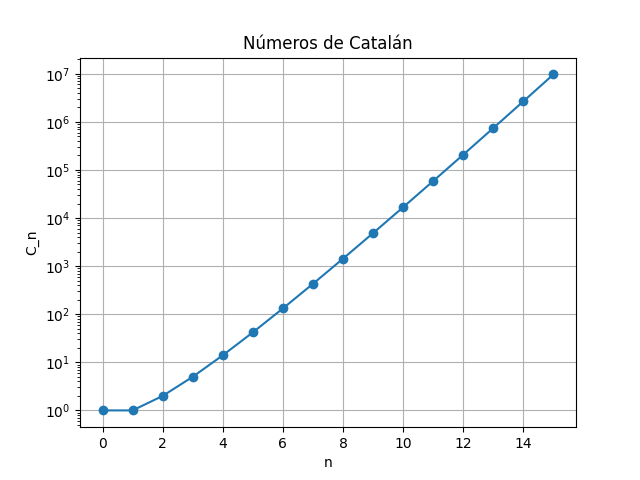
\includegraphics[width=\linewidth]{../img/Catalan_python.png}
    \caption{Utilizando solo funciones de Python.}
    \label{fig:min2}
  \end{minipage}
\end{figure}

Pero esta no es la forma mas eficiente de calcular los numeros de Catalan, ya que estamos calculando factoriales
muy grandes, lo que puede llevar a errores de overflow, como se vio en el caso de Numpy. Una forma mas eficiente
de calcular los numeros de Catalan es mediante el uso de las siguientes relaciones de recurrencia:

\begin{align}
    C_0 & = 1 \\ C_{n+1} = \frac{4n+2}{n+2}
\end{align}

Primero demostramos que $C_0 = 1$:

\begin{align}
    C_0 &= \frac{(2\cdot 0)!}{(0+1)! \cdot 0!} \\
        &= \frac{1}{1! \cdot 1} \\
        &= 1
\end{align}


Ahora, demostramos la segunda relacion de recurrencia:

\begin{align}
    \frac{c_{n+1}}{c_n} &= \frac{\frac{(2(n+1))!}{(n+2)! (n+1)!}}{\frac{(2n)!}{(n+1)! n!}} \\
                        &= \frac{(2n+2)!}{(n+2)! (n+1)!} \cdot \frac{(n+1)! n!}{(2n)!} \\
                        &= \frac{(2n+2)! \cdot n!}{(n+2)! (2n)!} \\
                        &= \frac{(2n+2)(2n+1)(2n)! \cdot n!}{(n+2)(n+1) n! (2n)!} \\
                        &= \frac{(2n+2)(2n+1)}{(n+2)(n+1)} \\
\end{align}

Por lo tanto, tenemos que:

\begin{equation}
    C_{n+1} = \frac{4n+2}{n+2} \cdot C_n
\end{equation}

Ahora implementando esta relacion de recurrencia en Python, tenemos el siguiente codigo:

\begin{lstlisting}
    import numpy as np
    import matplotlib.pyplot as plt

    N = 15
    cats = [0] * (N + 1)
    cats[0] = 1

    for n in range(N):
    cats[n + 1] = (4 * n + 2) * cats[n] // (n + 2)

    x = list(range(N + 1))
    y = cats

    plt.plot(x,y, "o-")
    plt.ylabel("$C_n$")
    plt.xlabel("$n$")
    plt.title("Números de Catalán")
    plt.yscale("log")
    plt.grid()
    plt.show()  
\end{lstlisting}

Y graficando los resultados obtenemos:

\begin{figure}[ht]
  \centering
  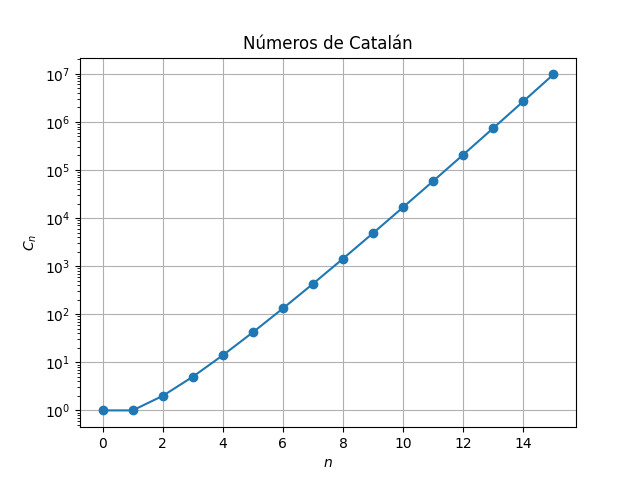
\includegraphics[width=0.65\textwidth]{img/Catmejor.png}
  \caption{Numeros de Catalan con la nueva implementacion.}
  \label{fig:catalan_mejor}
\end{figure}

\section*{Agradecimientos}

Gracias copilot

\end{document}